\documentclass{llncs}
\usepackage{llncsdoc}
\usepackage{amsmath}
\usepackage{algpseudocode}
\usepackage{algorithm}
\usepackage{algorithmicx}
\usepackage{color}
\usepackage{gnuplottex}
\usepackage{graphicx}
\usepackage{subcaption}
\captionsetup{compatibility=false}

%\algloopdefx[IfContinue]{IfContinue}
%[1]{\textbf{if} #1 \textbf{then break}}

\algsetblockdefx[IfContinue]{IfContinue}{IfContinue}
{0}{0pt}
[0]{}
[1]{\textbf{if} #1 \textbf{then continue}}

\begin{document}

\title{Encoding Reduce-Fold Cellular Automata for Distance Metrics using MDL}
\titlerunning{Encoding Reduce-Fold Cellular Automata}
\author{Micky E. Faas}
\institute{Leiden Institute of Advanced Computer Science \\ \email{micky@edukitty.org}}
\maketitle

%\begin{abstract}
%\end{abstract}
\bigskip

\section{Introduction}
Cellular automata are a class of discrete models first described in the 1940s by John von Neumann and Stanislaw Ulam\cite{neumann}. These automata are generally recognized for having the capability of exhibiting complex behavior given only a small set of \emph{rules} and inputs. The most influential research on this topic was done in the 1970s by John Conway and in the 1980s by Stephen Wolfram, about \emph{Game of Life}\cite{life} and \emph{elementary cellular automata}\cite{elemca}, respectively. A specific rule of the latter was later also proven\cite{cook} to be Turing-complete, which is just one of the many examples showing how cellular automata can be meaningful to computer science beyond their aesthetics.

In this essay, a variant developed by the author called the \emph{reduce-fold cellular automaton} is studied. First of all, the concept of this class of automata is introduced. After this, the problem of the very large rule space of these automata is described and how it impedes its further study. An approach to encoding and extracting structural information is then discussed, concluded by some preliminary experimental results.

\subsection{The Reduce-Fold Cellular Automaton}
A reduce-fold cellular automaton or \emph{RFCA} is discrete system with an output that resembles the structure of a tree. The system can be specified as a tuple $A=<b,m,r,\delta,S>$, where $b$ is the \emph{base}, $m$ is the \emph{mode} (neighbourhood size) and $S$ is a string that contains the input. $r$ specifies the {rule}, while $\delta$ is a set of \emph{reduction rules}. As these last two follow from each other, one can be omitted at any time.

An RFCA has two states of operation, namely \emph{reduction} and \emph{folding}. Both operations combined produce a triangular-shaped output that resembles a tree and is defined as $A'(i,j)$, where $i$ is a row within the output and $j$ is a column within row $i$. At any time, $k$ is the total number of rows and $A'(0)$ and $A'(k-1)$ denote the first and the last row respectively. The length of a row is given by $l(i) = l(0)-i(m-1)$, $l(0)$ being the length of the first row.
\subsubsection{Reduction} is an operation where a set $P$ of $m$ adjacent nodes is mapped onto one new node $C$. The value of this resulting node is determined by the transition table $\delta$ and depends on the values of the nodes in $P$. The transition table is just a set of $b^m$ mappings in the form of $<p_0,..,p_{m-1}> \to c$, where both $p_x$ and $c$ are numbers on the interval $[0;b)$, $b$ being the base of the automaton. 

The transition table $\delta$ can be obtained from the rule $r$ and vice versa in the same way as one does for elementary cellular automata, using Wolfram-code\cite{elemca}. First, the number $r$ is converted to a number in base $b$ where each digit $r_b,x$ is also a base-$b$ number and can be enumerated starting from the least-significant digit $r_0$. Then the list of transitions is constructed such that $<0,..,0_{m-1}> \to r_b,0$ up until $<b,..,b_{m-1}> \to r_{b,b^m}$.

To give a small example, take the case where $m=b=2$. For convenience, we will categorize all automata by their base and mode as $m.b$. So in the case $m=b=2$, we speak of class 2.2. In this class, there are $b^m=2^2=4$ possible transitions per rule. Now take for example rule $r=3$: in base $b$ (binary) form this is written as $r=0011_2$. Therefore, the transition table looks like this: $<0,0>\to1;<0,1>\to1;<1,0>\to0;<1,1>\to0$

The example above shows that given a class $m.b$ there are clearly $b$ different values possible for each of the $b^m$ transitions. This means that for any class there are $b^{b^m}$ possible rules. Each specific rule is denoted along with its class as $m.b.r$, so for example the automaton in the example above would be identified as $2.2.3$.

\subsubsection{Folding} is an operation where the final reduction step is used to expand the input row by one node. The final reduction step is the reduction of a row with a length $\geq m$ to row $k-1$ with a length $<m$. After this, no more reductions can be performed. By taking either the left-most or the right-most (depending on the direction of folding) node from the last row and placing it on the input row at the opposite side, however, exactly $k$ reductions yield $k$ new nodes at the \emph{running edge} of the triangle. The running edge (as opposed to the \emph{folding edge}) is the side of the triangle of the direction of the folding. This can be either left- or right folding -- expanding the input row to the left or to the right respectively.

When folding left\footnote{When folding to the right this operation is exactly mirrored.}, the right-most node of the final row $\beta = A'(k-1,l(k-1)-1)$ is copied to a position before the left-most node on the input row $A'(0,0)$. We call node $\beta$ a \emph{pivot}, while we denote the node at the right end of the input row $\alpha=A'(0,l(0)-1)$ as the \emph{apex}. By thinking of folding not as `copying' but rather as `physically folding' the pivot over to the input row, one could say that the shape of the automaton's output is a three-dimensional cone (with apex $\alpha$) rather than a triangle. As each fold also adds one row (by further reduction), this cone extends infinitely.

A visualisation of the reduce-fold cellular automaton and all its parameters is also available in the RFExplore application\cite{rfexplore}.

\subsection{Studying RFCA}
One of the questions in studying RFCAs is whether the different rules exhibit interesting properties. We know for example from elementary cellular automata, that many rules conform to certain functions, integer sequences\cite{elemca} or are even Turing-complete\cite{cook}. Sharing many of the mechanics with these systems RFCAs undoubtedly exhibit similar characteristics. Rather than looking at all different rules manually it would be preferable to have this task at least partly automated.
One of the main reasons for this being the fact that the rule space for some of the larger classes is immensely vast. Recall that the size of the rule space is given by $b^{b^m}$. For example, classes 2.2 and 3.2 have only 16 and 256 rules respectively while class 2.3 has 19,683 rules, class 2.4 has 4,294,967,296 rules and class 3.3 has 7,625,597,485,000 rules.

Many of the rules in these rule spaces are equivalent in some way. Wolfram already identified \emph{mirrored}, \emph{complementary} and \emph{amphichiral} rules\cite{elemca}. However, even many more rules exhibit \emph{structural similarity} while not being exactly structurally the same. Only by detecting these structures can we hope to map a rule space in a semantically meaningful way.

This mapping could be by the way of \emph{clustering} a rule space based on some distance metric. This distance metric should define a meaningful semantic or structural relation for two rules from the same class. One could hypothesize that the very small clusters contain rules with unique behaviour that are worth further study, while the bigger clusters probably contain mostly oscillating or terminating patterns.

\subsection{Clustering RFCA using MDL}
One of the possibilities in clustering RFCAs is by taking a finite part of the output $A'$ for a certain rule and input, and try to compare it structurally to same-length outputs from other rules. To this end we could employ existing pattern mining techniques as well as existing clustering methods such a \emph{k-Nearest Neighbour}. In this essay we propose a method using the \emph{Minimum Description Length}- or \emph{MDL} principle\cite{mdl}. MDL is a practical application of \emph{Kolmogorov complexity}\cite{kolmogorov}\cite{chaitin} which defines the complexity of a certain piece of data (object) as the length of the simplest program that generates this data. If such a program can also generate another object with minimal modifications, both objects must be very similar.

Chaitin's incompleteness theorem shows that Kolmogorov-complexity can only be used in theory and such a `simplest program' is not computable for any practical application. We therefore use a \emph{two-part MDL} as a practical approximation of Kolmogorov-complexity. The idea behind two-part MDL is to try to approach this simplest program from Kolmogorov-complexity by searching for a model $H$ that  encodes the given data best. This model $H$ should ideally reduce the data length by a large factor if the data contains little entropy, e.g. many repetitive structures. On the other hand, the reduction of the data length should not come at the expense of a very large model (or even a model containing all the data), because this leads to \emph{over fitting}. Therefore, in MDL the model length and the \emph{encoded data} length are considered together and we simply need to minimize the following function:
\begin{align*}
L(H) + L(D|H) \ .
\end{align*}
Where $L(H)$ is the length of the model and $L(D|H)$ is the (encoded) data given the model.

The approach using MDL has many advantages. First of all, there is no way of overfitting the data and there is no prior approximation or training required -- an encoding algorithm with MDL can essentially be parameter-free. Furthermore, the encoding of the data is loss-less which means we can reconstruct the data again from the model, but this also means the structure of the data is preserved within the model. Perhaps an even bigger advantage is that we can separate the structure (the model) from the parameters or \emph{residuals} (the encoded data). By applying the model of one object to another object we can measure their similarity by measuring the length of the encoded data. This not only gives a quantitative measure, but also tells \emph{how} the objects are different, e.g. which structures are in it and which not. Both measurements can play a crucial role in clustering.

While MDL has many benefits it also comes at the price of finding such model $M$. Finding the optimal model is computationally very hard for most problems. In many cases the search space is irregular, discontinuous and exponentially related to the input length. Therefore, many implementations using MDL employ some form of a greedy algorithm to find a `good' model instead of the most optimal. One way of approaching this is to find a suitable code that encodes the data very efficiently. This is essentially a form of compression and thus this type of data mining is often called `data mining by compression'.

\subsection{VOUW}
The first step in clustering RFCA is to obtain a distance metric that takes the automaton's structure into account. Using the MDL principle this means an algorithm is needed that is able to compress a given automaton's output or at least compute the \emph{length} of the compressed result. While a generic compression algorithm could be used, for example LZW or even JPEG, we would lose the ability to compress one rule's output with the code from another. Also, because the generic algorithms would merely be a black box to us, we would lose the ability to generate a qualitative measure. To reap all benefits from the MDL approach, a domain-specific encoding is required.

In this essay the author proposes the \emph{VOUW}\footnote{\emph{Vouw} is the Dutch translation for the word `fold'.} algorithm that attempts to encode the structures found in RFCA. VOUW has a strong emphasis on \emph{spatial relations} within the data and much less on the absolute values of different data points. This is a significant advantage when encoding RFCA, because the same structure can appear in different variations (e.g., inverted or mirrored). Take for example the structure of the string \texttt{1001} that has an equivalent structure to string \texttt{0110} while having a completely different absolute value. 

In VOUW, patterns of data points are encoded with a \emph{spatial offset} and a \emph{magnitude offset}. A set of these offsets represents a \emph{pattern}. One pattern can occur at different spatial locations or \emph{pivots} in the data and can have different \emph{variants}. In the example above, the strings would be encoded as $<0110,0>$ and $<0110,1>$ -- being a variant of the same pattern.
A tuple of a pivot, a pattern and variant is then called a \emph{region}. An encoded data set is a set of regions that completely cover the original data space in a non-overlapping fashion. Using this set of regions, the original data can be restored unambiguously. All patterns are also stored in a \emph{code table} that can be used to encode different data to obtain distance metrics. The VOUW algorithm uses a greedy approach to find a `good' set of patterns and regions that compress the data efficiently. The exact algorithm is described in Section \ref{encoding}.

\subsection{Related work}
The MDL principle has been employed in datamining of a wide variety of subjects. Important work include those by Vreeken et al.\cite{krimp} and Smet et al.\cite{slim}, describing the Krimp and SLIM algorithms respectively. Both algorithms are \emph{frequent item set} miners that employ a greedy MDL approach and serve as an inspiration for the algorithm in this essay.

Other subjects include event sequences such as the work by Tatti et al.\cite{tatti} and association of two-view data in work by Van Leeuwen et al.\cite{leeuwen}.
Lastly, the work Prakash et al.\cite{prakash} is worth mentioning as it also deals with 2-dimensional structural data by predicting the origin of epidemics. 



\section{VOUW}\label{encoding}
This section describes the VOUW encoding algorithm in detail. The input is given as a matrix or a function with two arguments $A'(i,j)$ mapping row $i$ and column $j$ to the automaton's output in node $(i,j)$ of a total of $|A'|$ nodes. The length of a row is given by $l(i) = l(0)-i(m-1)$, $l(0)$ being the length of the first row. Lastly, $b$ is the base of the automaton meaning that any magnitude will be on the interval $[0;b)$. First, let us begin with some important definitions.

A \textbf{pattern} is a set of tuples in the form $<\mathbf{v},w>$ , where $\mathbf{v}$ is an n-dimensional spatial offset within $A'$ and scalar $w$ is a magnitude offset.
A \textbf{region} is a set of tuples in the form $<X,t,\mathbf{q}>$, where $X$ is a pattern and $\mathbf{q}$ and $t$ are a pivot and a variant respectively. For the sake of brevity, we denote such a variant of a pattern as $X+t$. 

The set $A^{C}$ is the set of all regions that together encode $A'$.
The code table $C$ is a list of all patterns $X$ that occur in $A^C$. For each pattern the code table stores the usage (the number of times it occurs in $A^{C}$) and the code length. The code length is the theoretic number of bits that would be required to store one instance of $X$. It is defined by the probability $P(X)$ that $X$ occurs in $A^{C}$ by Shannon's Entropy\cite{shannon} $-\log P(X)$. Therefore, codes that are used very often will be smaller. A result is that rarely used patterns are discouraged by MDL through the fact that they make the code table (`model' in MDL-terms) more bulky.

Lastly we define \emph{gain} as the number of bits with which the total length $M(H)+M(D|H)$ is reduced. Gain plays an important role when searching for optimal candidate patterns, but can also be tricky to compute. Because of the way in which VOUW merges its patterns however, it is possible to give the exact gain for a combination in constant time.

\subsection{Finding candidates}
The algorithm begins by initializing the code table $C$ with only one singleton pattern $X_0=\{<0,0>\}$. $A'$ is then encoded using $X_0$ which results in exactly $|A'|$ different regions. The value of each node is encoded in the corresponding region's variant $t$. Since $P(X_0)=1$, the length of the code table is zero. 

The main goal of the algorithm is now to iteratively find pairs $X,Y$ of patterns of which the union $X \cup Y$ has the largest gain. However, a union also requires a relative distance $\delta$ between the patterns and a variant for each pattern. We therefore look for combinations of two regions instead of two patterns. Say region $<X,t,\mathbf{q}_x>$ and $<Y,s, \mathbf{q}_y>$ are considered, then the patterns $X+t$ and $Y+s$ are tested with $\delta = \mathbf{q}_y - \mathbf{q}_x$. The union is now given by:
\begin{align*}
X+t \ \cup \  Y+s+\delta &= \{<\mathbf{v}_x,w_x>,...\}+t \ \cup \  \{<\mathbf{v}_y,w_y>,...\} +s+\delta \\
 &= \{<\mathbf{v}_x,w_x+t>,...,<\mathbf{v}_y+\delta,w_y+s>,...\}\ .
\end{align*}

\subsection{Computing usage}
After a candidate union is computed\footnote{Note that in any practical implementation no actual union has to be computed as it suffices to remember the best combination of two patterns and two variants} it is tested for its ability to describe the data. Because of the way regions are stored, VOUW does not use the actual data to do any computations and rather uses the list of existing regions. As this list becomes smaller after subsequent steps of encoding, this process rapidly decreases in complexity.

The first measure that is computed is the usage for the pattern $X \cup Y$. Given that this pattern is composed of $X+t$ and $Y+s$, only regions containing those patterns have to be considered. The usage of $X\cup Y$ is therefore defined as:
\begin{align*}
\mathrm{usage}(X\cup Y) = |\{a,b \in A^C \ | \ X_a=X \land t_a=t \land X_b=Y \land t_b=s \land \mathbf{q}_b-\mathbf{q}_a = \delta\}| \ .
\end{align*}
Where $a$ and $b$ are tuples in the form of $<X,t,\mathbf{q}>$. Note that for a singular usage of an existing pattern we can simply define $\mathrm{usage}(X)=|\{a \in A^C | \ X_a=X \}|$.

\subsection{Computing gain}
In the case that $X\cup Y$ is accepted, only patterns $X$ and $Y$ will see a decreased usage, which makes computing the gain very easy. First of all, however, let us define the way the length of the code table $C$ ($L(H)$ in MDL terms) and the encoded regions $A^C$ ($L(D|H)$ in MDL terms) are computed. For every pattern, the code length is given by its probability to occur in $A^C$. For a pattern $X$ this is $P(X) = \frac{1}{\mathrm{usage}(X)}$ so the code length is $-\log P(X)$. To encode a pattern in the code table the variant also needs to be encoded. To not put any bias towards the variants of a pattern, the variant is encoded with a fixed length that is determined by the base $b$ as $\log b$. When encoding the pattern is the code table, the size of the pattern also influences the length of entry. For each offset, another $\log N$ ($N$ being the total number of nodes) bits is required. This makes the total sum for pattern's code table entry:
\begin{align*}
Lc(X) = -\log P(X) + |X| \log N \log b \ .
\end{align*}
To encode one region a similar sum is used. Instead of a list of offsets the pivot must be encoded, which also takes $\log N$ bits. This gives:
\begin{align*}
Lr(X) = -\log P(X) + \log N + \log b \ .
\end{align*}
Given $\mathrm{usage}(X\cup Y)$ we can now compute the gain of merging patterns $X$ and $Y$. First of all, the usages of $X$ and $Y$ are decreased by $\mathrm{usage}(X\cup Y)$. This increases the code lengths of both patterns which must be reflected by the gain. Additionally, if the usage of either $X$ and/or $Y$ becomes zero, they can be removed from the code table. Let us define $\mathrm{g}(X,X\cup Y)$ as the bits that are saved by replacing $X$ with $X\cup Y$:
\[ \mathrm{g}(X,X\cup Y) =
  \begin{cases}
     \mathrm{usage}(X)Lr(X) & \quad \text{if }\mathrm{usage}(X)-\mathrm{usage}(X\cup Y)>0\\
     \mathrm{usage}(X)Lr(X) + Lc(X) & \quad \text{if }\mathrm{usage}(X)-\mathrm{usage}(X\cup Y)=0
  \end{cases}
\]
Analogous, the function $\mathrm{cost}(X\cup Y)$ can be defined as the number of bits required to add the pattern $X\cup Y$. Subsequently, we define $\mathrm{gain}(X,Y)$ as the net gain of merging $X$ and $Y$.
\begin{align*}
\mathrm{cost}(X\cup Y) &= \mathrm{usage}(X\cup Y)\Big(Lr(X\cup Y) + Lc(X\cup Y)\Big) \\
\mathrm{gain}(X,Y) &= g(X,X\cup Y) + g(Y,X\cup Y) - cost(X\cup Y)
\end{align*}

\subsection{Encoding}
Given the functions defined in the previous paragraphs it is now possible to devise the algorithm \texttt{encode\_step} in Listing \ref{encodestep}. First, however, we describe a different method to compute the usage of a candidate pair of patterns. The usage function as described earlier has a complexity of $O(n^2)$ in the number of regions, making the total complexity of the algorithm unnecessary large ($O(n^4)$). As an alternative we define \texttt{USAGE} as a lookup-table that is indexed by a quadruple of the form $<X,Y,\delta,u>$ and maps to a single natural number representing the usage of that quadruple. In this case $u$ is the modulo difference between the variant of $X$ and the variant of $Y$. In a practical application \texttt{USAGE} can be implemented as perfect hash, BST or an array.

\begin{algorithm}
\caption{encode\_step()}
\label{encodestep}
\begin{algorithmic}
\State USAGE $\gets \emptyset$; candidates $\gets \emptyset$
\State unmask\_all$(A^C)$
\ForAll{$a \in A^C$} 
	\IfContinue{masked($a$)}
	\State $X \gets \mathrm{pattern}(a) $
	\State mask$(a)$
		\Comment Mask $a$ so it is not visited again
	\ForAll{$b \in A^C$}
		\IfContinue{masked($b$)}
		\State $Y \gets \mathrm{pattern}(b) $
		\State $\delta \gets \mathrm{pivot}(b) - \mathrm{pivot}(a)$
			\Comment Spatial relation
		\State $u \gets (\mathrm{variant}(b) + b - \mathrm{variant}(a)) \mod b$
		\State $c \gets <X,Y,\delta,t>$
		\If{USAGE$(c) = 0$} 
			\State candidates $\gets$ candidates $\cup \ c$
		\EndIf
		\State $\mathrm{USAGE}(c) = \mathrm{USAGE}(c) + 1$
	\EndFor
\EndFor
\State bestGain $\gets 0$; bestCandidate $\gets nil$
\ForAll{$<X,Y,\delta,u> \in candidates$}
	\State usage$(X\cup Y) = \mathrm{USAGE}(<X,Y,\delta,u>)$
	\If{gain$(X,Y) > $ bestGain}
	\State bestGain $\gets$ gain$(X,Y)$
	\State bestCandidate $\gets <X,Y,\delta,u>$
	\EndIf
\EndFor
\If{bestGain $> 0$}
	\State merge\_patterns$($ bestCandidate $)$; compute\_lengths()
\EndIf
\State \Return{bestGain}
\end{algorithmic}
\end{algorithm} 

\begin{algorithm}
\caption{merge\_patterns($X,Y,\delta,u$)}
\label{mergepatterns}
\begin{algorithmic}
\ForAll{$a \in A^C$} 
	\IfContinue{pattern$(a) \neq X$}
	\ForAll{$b \in A^C$}
		\IfContinue{pattern$(b) \neq Y$}
		\State $\delta' \gets \mathrm{pivot}(b) - \mathrm{pivot}(a)$
		\State $u' \gets (\mathrm{variant}(b) + b - \mathrm{variant}(a)) \mod b$
			\Comment Variant from $a$ to $b$
		\If{$\delta'=\delta \land u'=u$}
			\State $t \gets (\mathrm{variant}(a) + b - \mathrm{variant}(X)) \mod b$
					\Comment Variant from $X$ to $a$
			\State $q \gets \mathrm{pivot}(a)$
			\State $A^C \gets (A^C \cap a ) \cap b$
				\Comment Remove regions $a$ and $b$
			\State $A^C \gets A^C \cup <X\cup Y,t,q>$
				\Comment Create a new region for $X\cup Y$ at $q$
			\State usage$(X) \gets$ usage $(X)-1$; usage$(Y) \gets$ usage $(Y)-1$;
		\EndIf
	\EndFor
\EndFor
%\State prune\_pattern$(X)$; prune\_pattern$(Y)$
%	\Comment Remove a pattern if it's usage is zero 
\end{algorithmic}
\end{algorithm} 

The algorithm in Listing \ref{encodestep} consists of two parts: the first part builds a list of all candidates and implicitly computes their usage. This section has a complexity of $O(n^2)$ in the number of regions\footnote{Had we used the naive usage function described earlier the complexity would be $O(n^4)$.}. The second part computes the gain for each candidate and selects the promising one by iterating once over the list. On the third to last line the procedure \texttt{merge\_patterns} removes all regions that match the candidate $<X,Y,\delta,u>$ and creates new regions for $X\cup Y$ that cover the same nodes. Pseudo code for this procedure is listed in Listing \ref{mergepatterns}. Notice that while the variant $u$ from $X$ to $Y$ is given, yet another variant from the new region to the region it replaces has to be calculated in order to obtain the correct values for the nodes it encodes.

The name \texttt{encode\_step} already suggests that the encoding is performed in an iterative manner. As long as the value for \texttt{bestGain} is positive the encoding will continue. This is a very greedy approach: once a new pattern is added it will not be reconsidered. This means that the optimal encoding is never found and that there is a chance the algorithm will get stuck in a local minimum. A possible way to alleviate this is to implement a form of pruning as described by \cite{krimp} and \cite{slim}. With pruning, after each iteration all patterns in the code table are reconsidered by taking the gain of removing them and replacing them with other patterns or the singleton pattern. The idea is that patterns with a very small usage probably take more space than they save. From experiments, however, it was clear that in VOUW pruning would give negligible improvement.

\section{Experiments}

Two experiments are performed in order to assess the quantitative (how well it compresses) and qualitative (if relevant structures are found) aspects of VOUW. In the first experiment the entire classes 2.3 and 3.2 of RFCA are encoded and the compression ratio for each rule is recorded. To each automaton the same input \texttt{00110} or \texttt{2001122102} -- that contains every possible pair of base 2 or 3 numbers respectively-- is provided and 20 additional folds are generated. This experiment gives a good impression of the quantitative aspect, but says little about the relevance of the structures in the code table. Therefore, in a second experiment, we look at the result of encoding each rule with every other rule's generated code table. For this we take the 2.2 class of RFCA as it is small enough to perform some naive clustering on and it is also easy to visually judge the quality of the clusters.

\subsection{Results}

Figure \ref{fig:results1} shows a plot of compression ratio in \% against the rule number. As can be seen, VOUW achieves a relatively strong compression troughout the rule space. The rules on the right sides of the spectra compress much better than the rest which can be explained by the fact that the rules on the far right side of the rules space contain very little structure. The encoding takes just over 145 minutes for 19,683 automata on a Core i7-4600U machine.

The results from the second experiment can be seen in Figure \ref{fig:results2}. The raw output is a distance matrix $D$ where each cell $i,j$ is determined by $\frac{L(A_x'|C_y)-L(A_x')}{L(A'_x)}$ gives the relative amount of additional bits required to encode $x$ with the code table of $y$. $L(A'_x|C_y)$ means here: the size of the automaton with rule $x$ compressed with the code table obtained from rule $y$.

While the distance matrix $D$ is already fairly symmetric, we compute $DD^t$ in order to obtain symmetric distances. As an additional step a hierarchical clustering is computed from this multiplied matrix and is printed in Figure \ref{figure:cluster}. While the data is still quite noisy, the resulting clusters appear to be reasonable when compared to manual clustering of the 2.2 rule space. 

\begin{figure}
\centering
\begin{subfigure}{\textwidth}
\centering
\begin{gnuplot}[terminal=pdf,terminaloptions=color]
    unset key
	set xrange [0:255]
	set xlabel 'Rule #'
	set ylabel 'Compression ratio %'
	plot 'ratio-3.2.txt' with lines
\end{gnuplot}
\caption{Compression ratio of the 3.2 rule space}
\end{subfigure}
\begin{subfigure}{\textwidth}
\centering
\begin{gnuplot}[terminal=pdf,terminaloptions=color]
    unset key
	set xrange [0:19682]
	set xlabel 'Rule #'
	set ylabel 'Compression ratio %'
	plot 'ratio-2.3.txt' with lines
\end{gnuplot}
\caption{Compression ratio of the 2.3 rule space}
\end{subfigure}
\caption{Result set 1, compression ratio}
\label{fig:results1}
\end{figure}

\begin{figure}
\centering

\begin{subfigure}{\textwidth}
\centering
\begin{gnuplot}[terminal=pdf,terminaloptions=color]
    unset key
	set autoscale xfix
	set autoscale yfix
	set autoscale cbfix
	plot '2.2.cluster.txt' matrix nonuniform with image
\end{gnuplot}
\caption{Distance matrix of the 2.2 rule space}
\end{subfigure}
\begin{subfigure}{\textwidth}
\centering
\begin{gnuplot}[terminal=pdf,terminaloptions=color]
    unset key
	set autoscale xfix
	set autoscale yfix
	set autoscale cbfix
	plot '3.2.cluster.txt' matrix nonuniform with image
\end{gnuplot}
\caption{Distance matrix of the 3.2 rule space}
\end{subfigure}
\caption{Result set 2, distance matrices}
\label{fig:results2}
\end{figure}

\begin{figure}
\centering
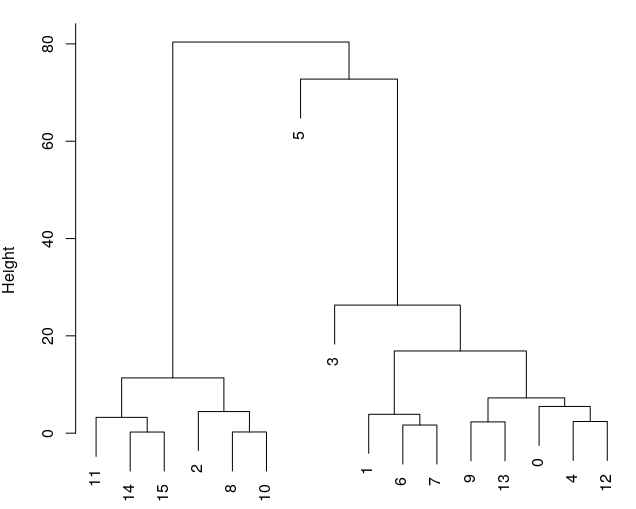
\includegraphics[scale=0.5]{cluster-2-2.png}
\caption{Hierarchical clustering of the 2.2 rule space}
\label{figure:cluster}
\end{figure}

\section{Conclusion}
The first results from VOUW look promising enough to warrant further study. Experiments have shown that actual structure from the data can be found through a greedy approach using MDL. Of course, it will have to be compared to other methods in order to really judge its value. For RFCA for example, another clustering method exists that only takes the transition tables into account.

While the algorithm described in this essay is designed to efficiently encode RFCA it can be used on other data as well, as long as it fits these requirements:
\begin{itemize}
\item Emphasis on n-dimensional structure.
\item Spatially discrete representation (e.g., a matrix) and discrete magnitudes.
\item Range of magnitudes known a priori and preferably small.
\end{itemize}
Examples of such data are MRI-images, graphs and any sort of (binary) matrices. While regular images may seem a good candidate, the structure detection in VOUW is not scale-invariant and would therefore have to be modified to operate on images.

It would be interesting to see how VOUW compares to other (MDL-based) methods of encoding the class of data mentioned above. Moreover, if scale-invariance could be added to VOUW it would be possible to measure its performance in computer vision applications.

\begin{thebibliography}{}

\bibitem{neumann}
Von Neumann, J. and A. W. Burks:
``Theory of self-reproducing automata."
Urbana, University of Illinois Press. (1966)

\bibitem{life}
Gardner, Martin:
``Mathematical Games -- The fantastic combinations of John Conway's new solitaire game ``life"". 
In: Scientific American. 223: 120–123. ISBN 0-89454-001-7.
(1970)

\bibitem{elemca}
Wolfram, Stephen:
``Statistical mechanics of cellular automata."
In: Reviews of Modern Physics, Vol. 55.3: 601--644.
(1983)

\bibitem{cook}
Cook, Matthew: 
``Universality in elementary cellular automata." 
In: Complex systems 15.1 (2004): 1-40.

\bibitem{mdl}
Rissanen, J: 
``Modeling by shortest data description". 
In: Automatica. 14 (5): 465–658.
(1978)

\bibitem{kolmogorov}
Kolmogorov, Andrey:
``On Tables of Random Numbers". 
In: Sankhyā Ser. A. 25: 369–375.
(1963)

\bibitem{chaitin}
Chaitin, Gregory J.: 
``On the Simplicity and Speed of Programs for Computing Infinite Sets of Natural Numbers". 
In: Journal of the ACM. 16 (3): 407–422.
(1969)

\bibitem{krimp}
Vreeken, J, van Leeuwen, M \& Siebes, A.:
``Krimp: Mining Itemsets that Compress."
In: Data Min. Knowl. Discov. 23(1):169-214.
(2011)

\bibitem{slim}
Smet, K \& Vreeken, J.:
``SLIM: Directly Mining Descriptive Patterns." 
In: Proceedings of the SIAM International Conference on Data Mining (SDM), pp 236-247
(2012)

\bibitem{tatti}
Tatti, N \& Vreeken, J.:
``The Long and the Short of It: Summarising Event Sequences with Serial Episodes."
In: Proceedings of the ACM SIGKDD International Conference on Knowledge Discovery and Data Mining (KDD), pp 462-470.
(2012)

\bibitem{leeuwen}
van Leeuwen, M \& Galbrun, E.:
``Association Discovery in Two-View Data. Transactions on Knowledge and Data" In: Engineering 27(12):3190-3202.
(2015)

\bibitem{prakash}
Prakash, B.A., Vreeken, J. \& Faloutsos: 
``Efficiently spotting the starting points of an epidemic in a large graph"
In: C. Knowl Inf Syst (2014) 38: 35.
(2013)

\bibitem{shannon}
Shannon, Claude E., and Warren Weaver.:
``The mathematical theory of communication.''
In: University of Illinois press. (1998)

\bibitem{rfexplore}
RFExplore, interactive visualisation of Reduce-Fold Cellular Automata \\
\texttt{https://github.com/mickymuis/rfexplore}

\end{thebibliography}

\end{document}